Mezní kmitočet navrhovaného filtru byl zvolen v řádu stovek kHz, což umožňuje využití např. pro přenos rozhlasového vysílání v atmosféře. Tyto dlouhé vlny (30 -- 300~kHz, čemuž odpovídá délka vlny 1 -- 10~km) obtékají nerovnosti a jdou za obzor bez nutnosti odrazu. Dnes na dlouhých vlnách vysílá jen několik národních rozhlasových vysílačů velkých států a pásmo se hlavně využívá pro takové účely, kde je na prvním místě spolehlivost a výhody pozemní vlny. To jsou například frekvenční a časové standardy (DCF77), radiomajáky, případně i komunikace s ponorkami. Střední vlny (525 -- 1705 khz, což odpovídá vlnovým délkám 186 -- 577 m) mají menší dosah a často u nich dochází k jednomu odrazu od atmosféry. Lépe se ohýbají za přírodními překážkami a jsou vhodné pro vysílání v okruhu stovek kilometrů. Mezní kmitočet filtru lze pomocí vstupnímu proudu tekoucímu do zesilovače měnit až v rozsahu několika dekád. 
\subsection{Analogové filtry}
Filtry jsou určeny k potlačení nebo zvýraznění určité části kmitočtového spektra signálu. Jsou to obvody s kmitočtově závislou přenosovou funkcí (pro napěťový přenos $H_s(j \omega) = U_{out}(j \omega)/U_{in}(j \omega)$). Základní rozdělení je na dolní propust (DP, anglicky \textit{low-pass} - LP), horní propust (HP, \textit{high-pass} - HP), pásmovou propust (PP, \textit{band-pass} - BP) a pásmovou zádrž (PZ, \textit{band-stop} - BS). \\
\\
Dolní propust nepropouští na výstup vstupní signál nad frekvencí $f_s$, signál v propustném pásmu zůstává beze změny nebo zesílený. Základní pasivní dvojbranné zapojení je ke vstupu sériově zapojený rezistor a k této větvi paralelně kapacitor. Tento RC člen (integrační článek) se zvyšující se frekvencí snižuje svou vstupní impedanci. Přenosová funkce má nulu v nekonečnu a pól v levé polorovině s-roviny. Ideální integrátor má pól v nule. \\
Horní propust nepropouští signály o nízkých frekvencích. Nejjednodušší zapojení je RC člen (derivační článek), kdy kapacitor je zapojen sériově se zdrojem a k této větvi paralelně rezistor. Pro toto zapojení reaktance kapacitoru se zvyšující se frekvencí klesá. Přenosová funkce ideálního derivátoru má pól v nekonečnu a nulu v nule. Horní propust má nulu v nule a pól v levé polorovině s-roviny.\\
\\
Pásmová propust propouští pásmo určené dvěma kmitočty. Pasivní pásmové propusti nedosahují účinnosti větší než 1. Jsou složeny z integračního článku (RC - dolní propust) a derivačního článku (CR - horní propust).\\
\\
Pásmová zádrž nepropouští kmitočty pásma definovaného dvěma kmitočty. Pasivní zapojení je složeno ze dvou rezistorů a kapacitorů. Má vždy ztrátový přenos.
\begin{figure}[h]
\centering
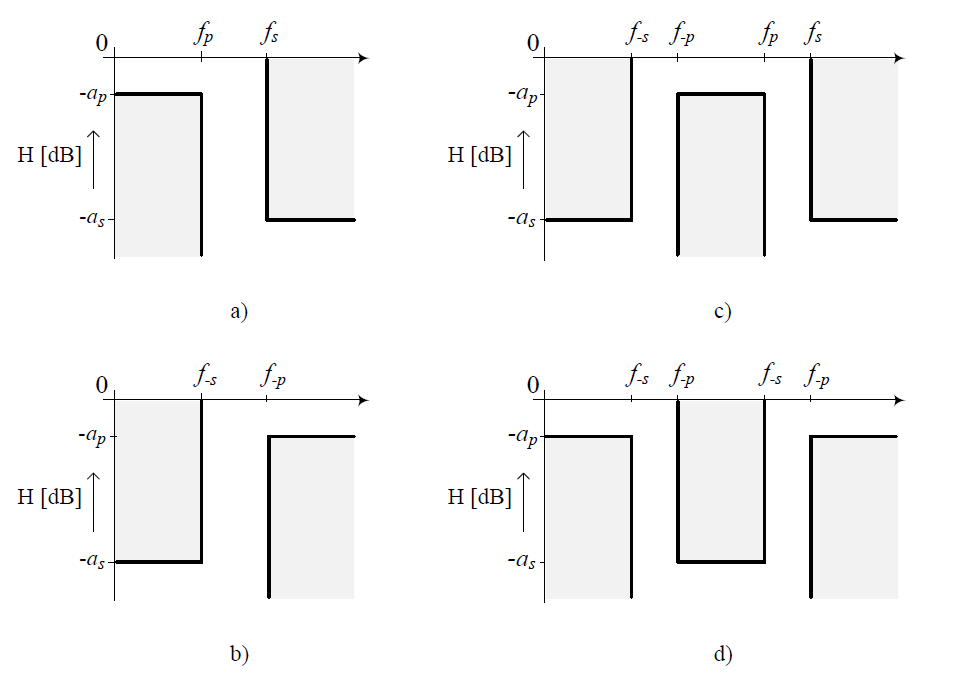
\includegraphics[scale=0.55]{tolerancnischemata.png}
\caption[Toleranční schéma dolní propusti (DP), horní propusti (HP), pásmové propusti (PP) a pásmové zádrže]{Toleranční schéma pro a) dolní propust (DP), b) horní propust (HP), c) pásmovou propust (PP) a d) pásmovou zádrž (PZ)\cite{1}}
\end{figure}
\noindent Filtry se používají k redukci nežádoucích frekvencí např. pro efektivní reprodukci zvuku reproduktory, k redukci okolního rušení - vysílače blokují harmonické frekvence, které interferují. Také v obvodech rekonstrukce signálů u D/A převodníků, k předvzorkování u A/D převodníku nebo jako anti-aliasing filtry.\\\\
Obecná přenosová funkce filtru typu dolní propust je
\begin{equation}
H(j\omega) = \frac{H_0}{\prod_{i=1}^{\frac{n}{2}} (1 + a_i s + b_i s^2)},
\end{equation}
kde $n$ je řád filtru.\\
Obecná přenosová funkce filtru typu horní propust je
\begin{equation}
H(j\omega) = \frac{H_{\infty}}{\prod_{i=1}^{\frac{n}{2}} (1 + \frac{a_i}{s} + \frac{b_i}{s^2})},
\end{equation}
kde $n$ je řád filtru.\\
Podle rozložení nul a pólů jmenovatele rozlišujeme různé aproximace. Koeficienty filtru $a_i, b_i$ určují zesílení v propustném pásmu. Činitel jakosti je definován jako $Q = \sqrt{b_i}/a_i$. Čím větší $Q$ je obdrženo, tím spíš bude filtr nestabilní.
\begin{figure}[h]
\centering
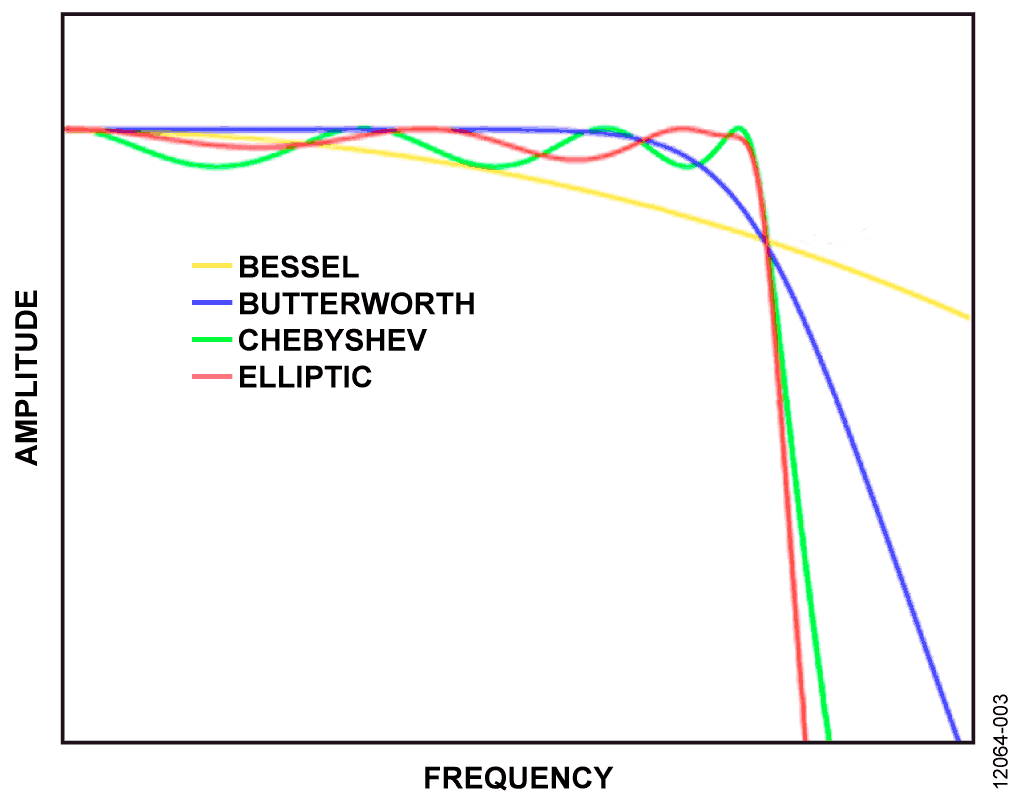
\includegraphics[scale=0.3]{LGA98.png}
\caption[Typy aproximací (DP)]{Typy aproximací (DP)\cite{2}}
\end{figure}
\subsection{Butterworthova aproximace}
Butterworthova má maximálně plochou amplitudovou charakteristiku v propustném pásmu. Frekvenční charakteristika má sklon daný počtem pólů a pro její posouzení je užíváno skupinové zpoždění (derivace fáze podle frekvence). Pro Butterworthovu aproximaci je skupinové zpoždění nezvlněné v propustném pásmu. Přechodová charakteristika má mírný překmit, zvyšující se s řádem filtru. Zesílení $G(\omega)$ je kmitočtově závislé a odpovídá absolutní hodnotě přenosové funkce $H(j\omega)$.
\begin{equation}
G(\omega) = |H(j\omega)| = \frac{1}{\sqrt{1 + \epsilon ^2 \frac{\omega}{\omega _c}^{2n}}},
\end{equation}
kde $\epsilon$ je poměrné zvlnění kmitočtové charakteristiky v propustném pásmu (\textit{faktor zvlnění}), $n$ je řád filtru a $\omega _c$ mezní kmitočet (nastává při útlumu -3 dB). Pro $\omega _c = 1$ je faktor zvlnění $\epsilon = 1$. 
\subsection{Čebyševova aproximace}
Čebyševova aproximace má strmější pokles, což vede k užití nižšího řádu filtru. Zato má ale zvlněnou frekvenční charakteristiku v propustném pásmu. 
\subsubsection{Typ I}
Vyjádření modulové charakteristiky pro tuto aproximaci je dáno jako
\begin{align}
G(\omega) = |H(j\omega)| = \frac{1}{\sqrt{1 + \epsilon ^2 T_n ^2 \frac{\omega}{\omega _c}^{2n}}},
\end{align}
kde $T_n$ je Čebyševův polynom, $\epsilon$ je poměrné zvlnění, $n$ je řád filtru a $\omega _c$ mezní kmitočet. Čebyševův polynom je definován vztahem $2 \omega ^2 - 1$ pro $n = 2$. Obecně jsou to kořeny Chebyshevových diferenciálních rovnic
\begin{align}
(1 - x^2)y" - xy' + n^2y &= 0\\
(1 - x^2)y" - 3xy' + n(n+2)y &= 0.
\end{align}
\subsubsection{Typ II}
Typ II je nazýván také jako inverzní Čebeševova aproximace. V praxi není příliš používaný, jelikož nemá tak rychlý pokles jako typ I a k jeho realizaci je třeba více prvků. Nemá zvlnění v propustném pásmu, zato v zádržném ano. Zesílení je definováno jako
\begin{equation}
G(\omega, \omega _c) = \frac{1}{\sqrt{1 + \frac{1}{\epsilon ^2 T_n ^2 \frac{\omega _c}{\omega}^{2n}}}},
\end{equation}
kde $T_n$ je Čebyševův polynom, $\epsilon$ je poměrné zvlnění, $n$ je řád filtru a $\omega _c$ mezní kmitočet.
\subsection{Besselova aproximace}
Besselova aproximace se používá v telekomunikační technice v případech, kdy je požadováno zachování tvaru signálu. Amplitudová charakteristika v nepropustném pásmu je velmi plochá. Koeficienty polynomu jsou zvoleny tak, aby fázová charakteristika v pásmu okolo kritické frekvence byla maximálně lineární. Nevýhodou je poměrně malá strmost modulové charakteristiky. Ta je pro Besselovu aproximaci dána vztahem
\begin{equation}
G(\omega) = |H(j\omega)| = \frac{\Theta _n(0)}{\Theta _n(\frac{j\omega}{\omega _c})},
\end{equation}
kde $\Phi _n$ je Besselův polynom a $\omega _c$ mezní kmitočet. Besselův polynom je definován součtem řady (Grosswald 1978, Berg 2000)
\begin{equation}
\Theta _n (x) = x^n y_n (\frac{1}{x}) = \sum_{k=0}^{n}\frac{(n+k)!}{(n-k)!k!}\frac{x^{n-k}}{2^k}.
\end{equation}
Pro filtr druhého řádu platí
\begin{equation}
G(\omega) = |H(j\omega)| = \frac{3}{\sqrt{\omega ^4 + 3\omega ^2 + 9}}.
\end{equation}
\subsection{Cauerova (eliptická) aproximace}
\noindent Cauerova aproximace (eliptická) má nejstrmější pokles, při jejím užití jsou voleny nižší řády filtru. Pokud se zvlnění v zádržném pásmu blíží nule, filtr se stává Čebyševovým (výše zmíněný - typ I). Opačně je tomu v propustném pásmu - přiblížením k nule se filtr stává inverzním Čebyševovým (typ II).  Pokud se obě hodnoty zvlnění blíží k nule, filtr se stává Butterworthovým. Kmitočtová charakteristika je dána vztahem
\begin{equation}
G(\omega) = |H(j\omega)| = \frac{1}{\sqrt{1 + \epsilon ^2 R_n ^2(\zeta, \frac{\omega}{\omega _c})}},
\end{equation}
kde $\epsilon$ je faktor zvlnění, $R_n$ eliptická racionální funkce n-tého řádu, $\zeta$ selektivní faktor a $\omega _c$ mezní kmitočet. Pokud pro selektivní faktor platí $\zeta \rightarrow \infty$, filtr se stává Čebyševovým (typ I).\\
Protože se, podobně jako u Čebyševovy aproximace, liší odvození pro liché a sudé stupně, jsou pro ně různé postupy. Pro lichý stupeň existuje pouze jedna varianta, pro sudý tři varianty (A, B, C), které se liší průběhem aproximační funkce.
\subsubsection{Cauerova (eliptická) aproximace typu A}
Má stejný počet pólů a nul aproximující funkce. Je realizována jako LC filtr (Sekce \ref{s:LC}) pouze s vázanými induktory.
\subsubsection{Cauerova (eliptická) aproximace typu B}
Jedná se o posun útlumového pólu z konečného kmitočtu k nekonečnu, tedy dále od propustného pásma. Tato úprava vede ke snížení strmosti přechodu od propustného k nepropustnému pásmu. Je to obdoba postupu u inverzní Čebyševovy aproximace.
\subsubsection{Cauerova (eliptická) aproximace typu C}
Vhodnou transformací, která vede na nulovou hodnotu přenosu v nulovém kmitočtu, získáme navíc proti variantám A, B i shodné zakončovací odpory v případě LC realizace (Sekce \ref{s:LC}). Je to obdoba postupu u Čebyševovy aproximace.
\subsection{Srovnání typů aproximací}
Z hlediska zápisu přenosové funkce není rozdíl mezi Butterworthovou a Čebyševovou aproximací, přestože jedna má v propustném pásmu hladký a druhá zvlněný průběh. Přenosová funkce má v čitateli konstantu a ve jmenovateli polynom (odtud společné označení polynomiální aproximace).\\
Oproti tomu volba průběhu v nepropustném pásmu tvar přenosové funkce mění. Pokud je průběh monotónní (Butterworthova, Čebyševova aproximace), jedná se o podíl konstanty a polynomu. Je-li průběh v nepropustném pásmu zvlněný, tvoří přenosovou funkci podíl dvou polynomů. Pro běžné aproximace (Cauerova, inverzní Čebyševova) je v čitateli sudý polynom ve tvaru $\prod _{i} (p^2 + \omega_i^2)$.\\
Volbou kombinace hladkého a zvlěného průběhu v propustném a nepropustném pásmu získáme různé vlastnosti.\\
 \begin{table}[h]
 \caption[Přehled aproximací podle tvaru aproximační funkce v propustném i nepropustném pásmu]{\label{tab:Přehled aproximací podle tvaru aproximační funkce v propustném i nepropustném pásmu}Přehled aproximací podle tvaru aproximační funkce v propustném i nepropustném pásmu \cite{3}}
  \end{table}
\begin{center}
\begin{table}[h]
\centering
  \begin{tabular}{ | c | c | c | }
    \hline
    Propustné pásmo & Nepropustné pásmo & Příklad aproximace \\ \hline
    hladká & hladká & Butterworthova \\ \hline
    zvlněná & hladká & Čebyševova \\ \hline
    hladká & zvlněná & inverzní Čebyševova \\ \hline
    zvlněná & zvlněná & Cauerova \\ \hline
  \end{tabular}
   \end{table}
   \end{center}